\subsection{Overview of the testbed}
% Although the algorithm performed well in the offline simulation, it is not enough just to validate the algorithm in an off-line environment. 
To validate the feasibility of the algorithm for practical use, real-time controller-hardware-in-the-loop (CHIL) simulation was performed. The CHIL testbed and python API presented in \cite{newaz2019controller} was used for the CHIL validation of the CVC algorithm. Fig. \ref{fig:CHIL_BLOCK} represents the block diagram of the CHIL setup. In the case of the real-time CHIL simulation, a more realistic scenario was considered. It was assumed that the real and reactive power information from the load points and the inverters were available. Also, the current status of the capacitor banks and OLTC was available. Finally, the voltage violation detection signal, as well as the current voltage magnitude and voltage angle at the substation, was available. Besides that, no other information was available from the system. A photograph of the actual CHIL setup is shown in Fig. \ref{fig:CHIL_SETUP}. The CHIL simulation setup consists of three major components.

\begin{figure}[!h]
\centering
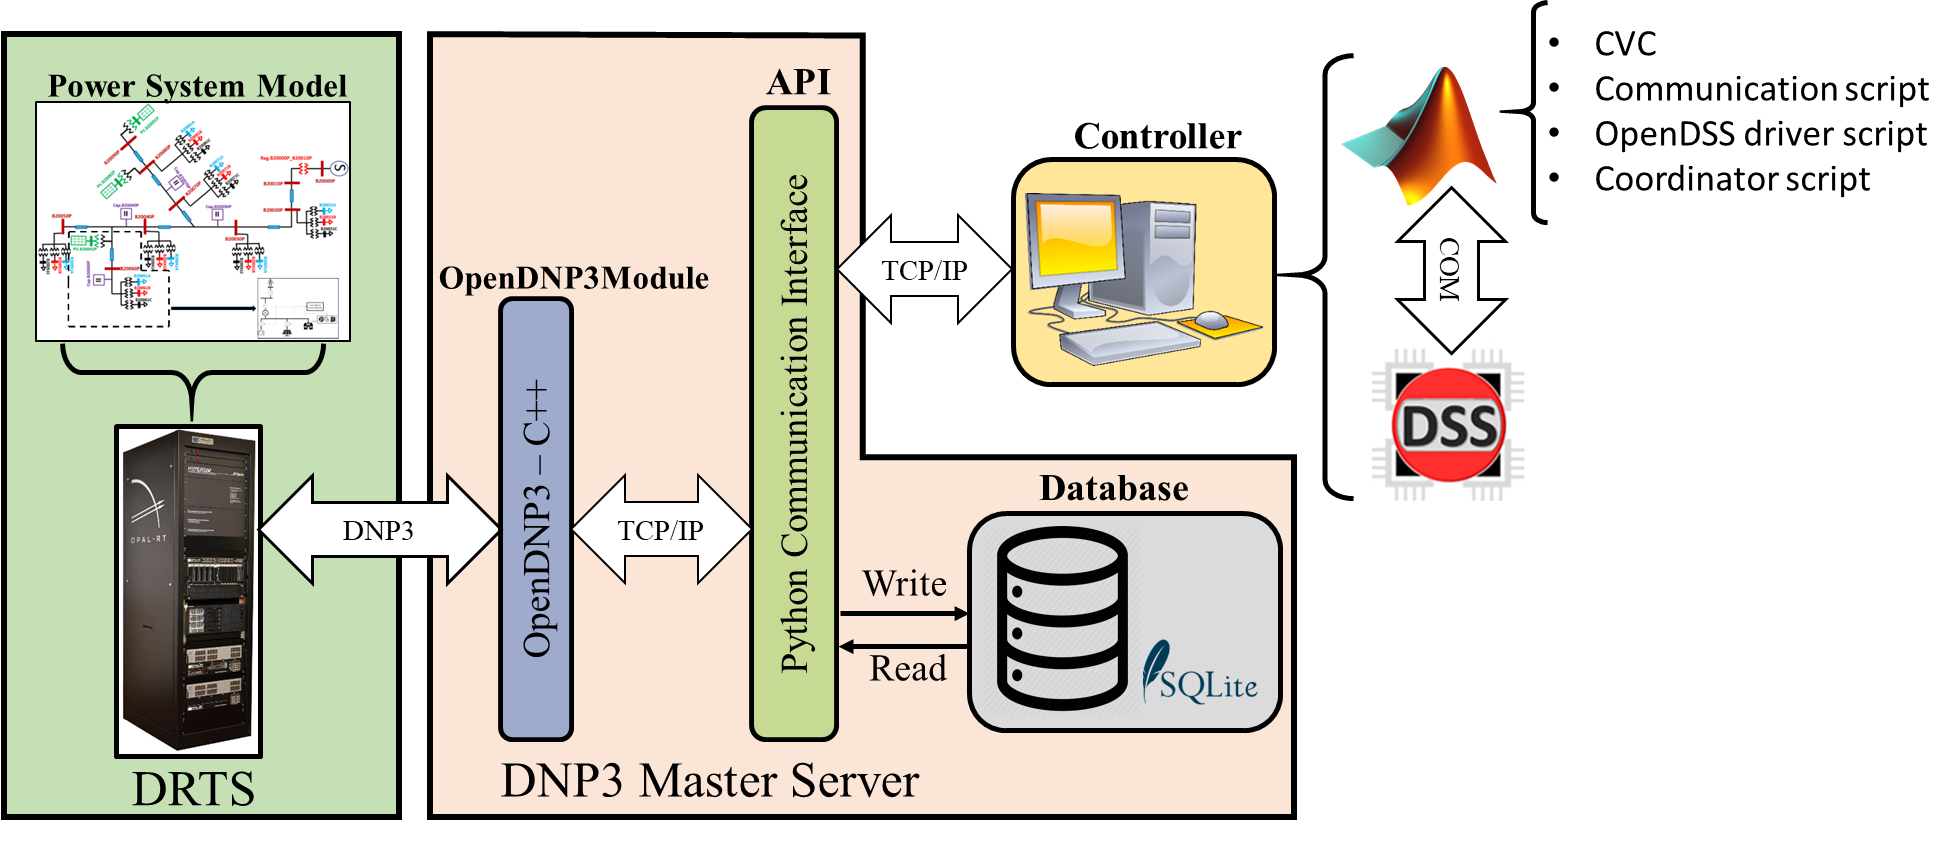
\includegraphics[width=\linewidth]{figs/RT_BLOCK_2.png}
\caption{Block diagram of the CHIL setup.}
\label{fig:CHIL_BLOCK}
\end{figure}


\begin{figure}[!h]
\centering
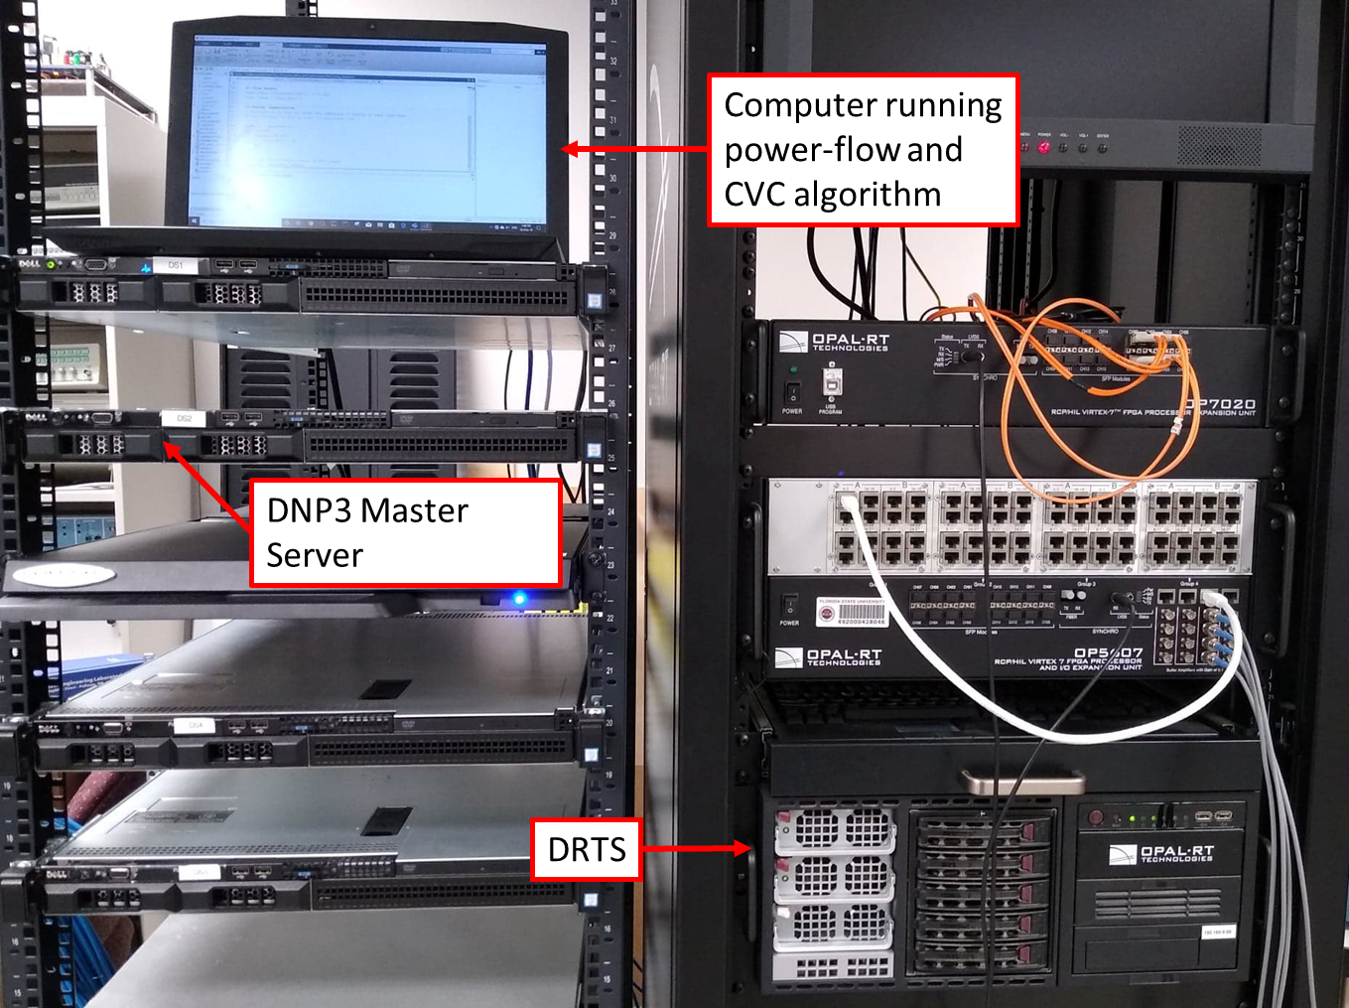
\includegraphics[width=\linewidth]{figs/LAB_SETUP.png}
\caption{Photograph of the CHIL setup}
\label{fig:CHIL_SETUP}
\end{figure}


\subsubsection{Power System Modeled in Digital Real-time Simulator (DRTS)}
It consists of different models designed to represent and simulate the behavior and interactions of grid-connected distributed energy resources (DERs) in a real-time environment. Some of these components are a) models of DERs (Lithium-ion batteries as energy storage systems (ES), Photovoltaic (PV) systems), b) dynamic load models designed to simulate dynamic loading conditions,  c) models of the distribution network and d) models of smart-meter devices designed to measure and communicate data such as voltages, currents, active power, and reactive power to the main (external) control system. All of these systems are modeled inside the digital real-time simulator (DRTS). 

\subsubsection{DNP3 Master Server}
The 'DNP3 Master Server' is in charge of sending and receiving data from the DRTS over DNP3. It also records the data and establishes connections with controllers.  It has the following main parts.
\begin{itemize}
    \item \textbf{OpenDNP3 C++} It consists of a real-world DNP3 communication infrastructure based on the OpenDNP3 \cite{opendnp3_2020} project. It communicates with the smart-meter models inside the DRTS via the IEEE 1815 DNP3 communication protocol. It also sends data back to the DRTS using DNP3 as well. It is programmed in C++ using OpenDNP3 as a base to enable DNP3 communication.
    \item \textbf{Python Communication Interface:} This consists of application programming interfaces (APIs) designed to provide inter-process communication to any generic control algorithm. They provide a communication bridge between the DNP3 communication module, a database management server, and any generic control algorithm devised to be deployed (and tested) in real-time system environments. The API is designed to work with SQL light databases. The API also allows any generic controller to send data to the communication layer to be sent to the DRTS.
    \item \textbf{Database} The database is there to store the data received over the DNP3 communication layer from the DRTS. In this implementation, an SQL light database was used. The 'Python Communication Interface' layer writes the data received over DNP3 in the database it also enables sending of the data to the outside control algorithm.
\end{itemize}

\subsubsection{Controller:}
The controller, in this case, is a computer running the power-flow and CVC algorithm. The CVC algorithm and power-flow are controlled using a coordinator script. This is a script written in the Matlab scripting language to communicate with the Controller-to-database API over TCP/IP and execute the various sections of the CVC algorithm in proper order. The coordinator script starts by running the communication script to receive the reinvent data from the DNP3 Master Server. Then it runs a power-flow using openDSS based on the current data. This is done by configuring and controlling the openDSS engine oven the Windows COM interface. After running the power-flow the coordinator script runs the CVC algorithm to get the reactive power compensation needed. And then it runs the communication script again to send the control actions back to the DNP3 Master Server over TCP/IP and the DNP3 Master Server relays the data to the DRTS simulation over DNP3.

\subsection{Real-time CHIL results}
The real-time simulation was run for 900 seconds using the system PV and load profile used in the offline simulation. The simulation uses the system profile from 38160s to 39060s. Fig. \ref{fig:RT_VVC} shows the whole real-time simulation voltage profiles. The dashed line represents the upper limit 'UL' of the voltage bounds. The rest of the legend uses the same notations as Fig.\ref{fig:with_cvc}. It can be seen in the figure that the real-time implementation of the algorithm is able to mitigate the voltage violation that occurs during the simulation.

\begin{figure}[!h]
\centering
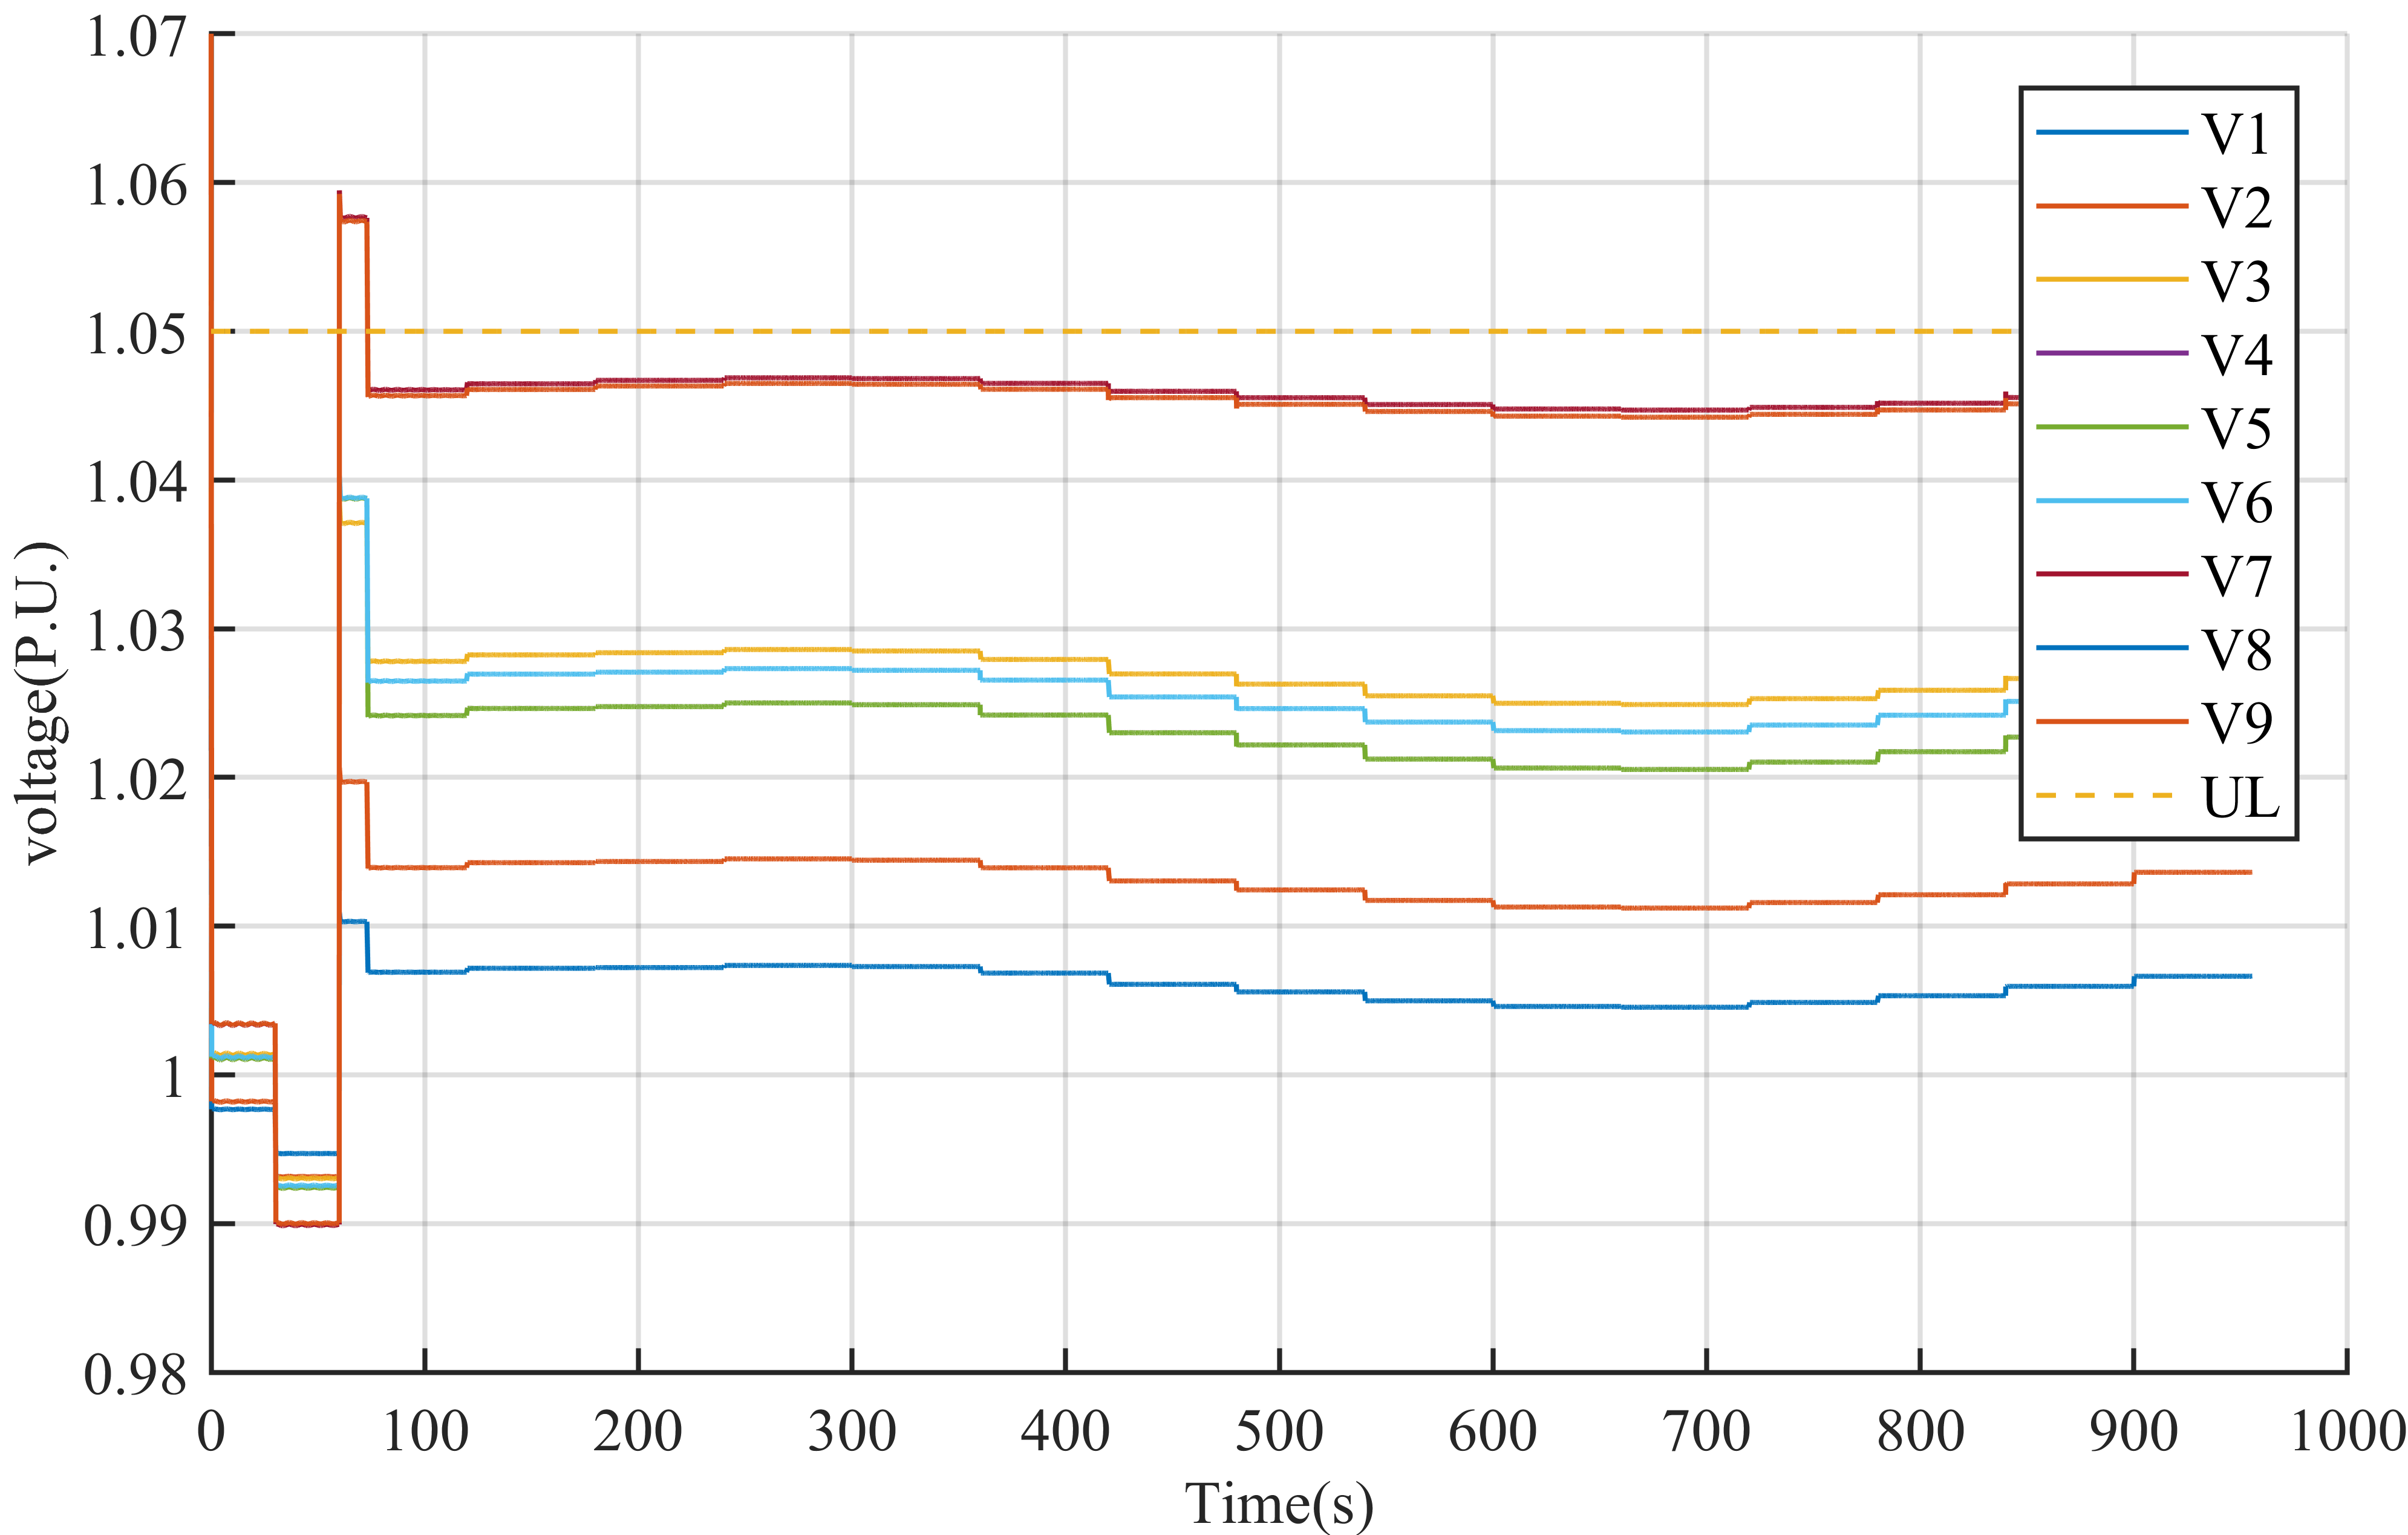
\includegraphics[width=\linewidth]{figs/RT_VOLTAGES.png}
\caption{Real-time voltage profile with coordinated voltage control.}
\label{fig:RT_VVC}
\end{figure}

\subsubsection{Real-time vs offline voltage profile}
Fig. \ref{fig:RT_VS_OFF_V} shows the voltage profile of 'V7' for both the offline and real-time simulation. 'V7' is chosen to be shown here because it shows the highest violation in the system for both offline and real-time simulations. The solid line represents the offline and the dotted line represents the real-time profile. It can be seen that the real-time simulation takes 11s to mitigate the voltage violation where the offline simulation took 2s. This is expected as the real-time simulation implements a real-world communication infrastructure with smart meters and a power-flow step to estimate the system status. This response time is comparable to the current voltage regulation schemes which take around 5s to 10s to coordinate system voltages. Other than that the offline and real-time profiles deviate less than 2\%. 

\begin{figure}[!h]
\centering
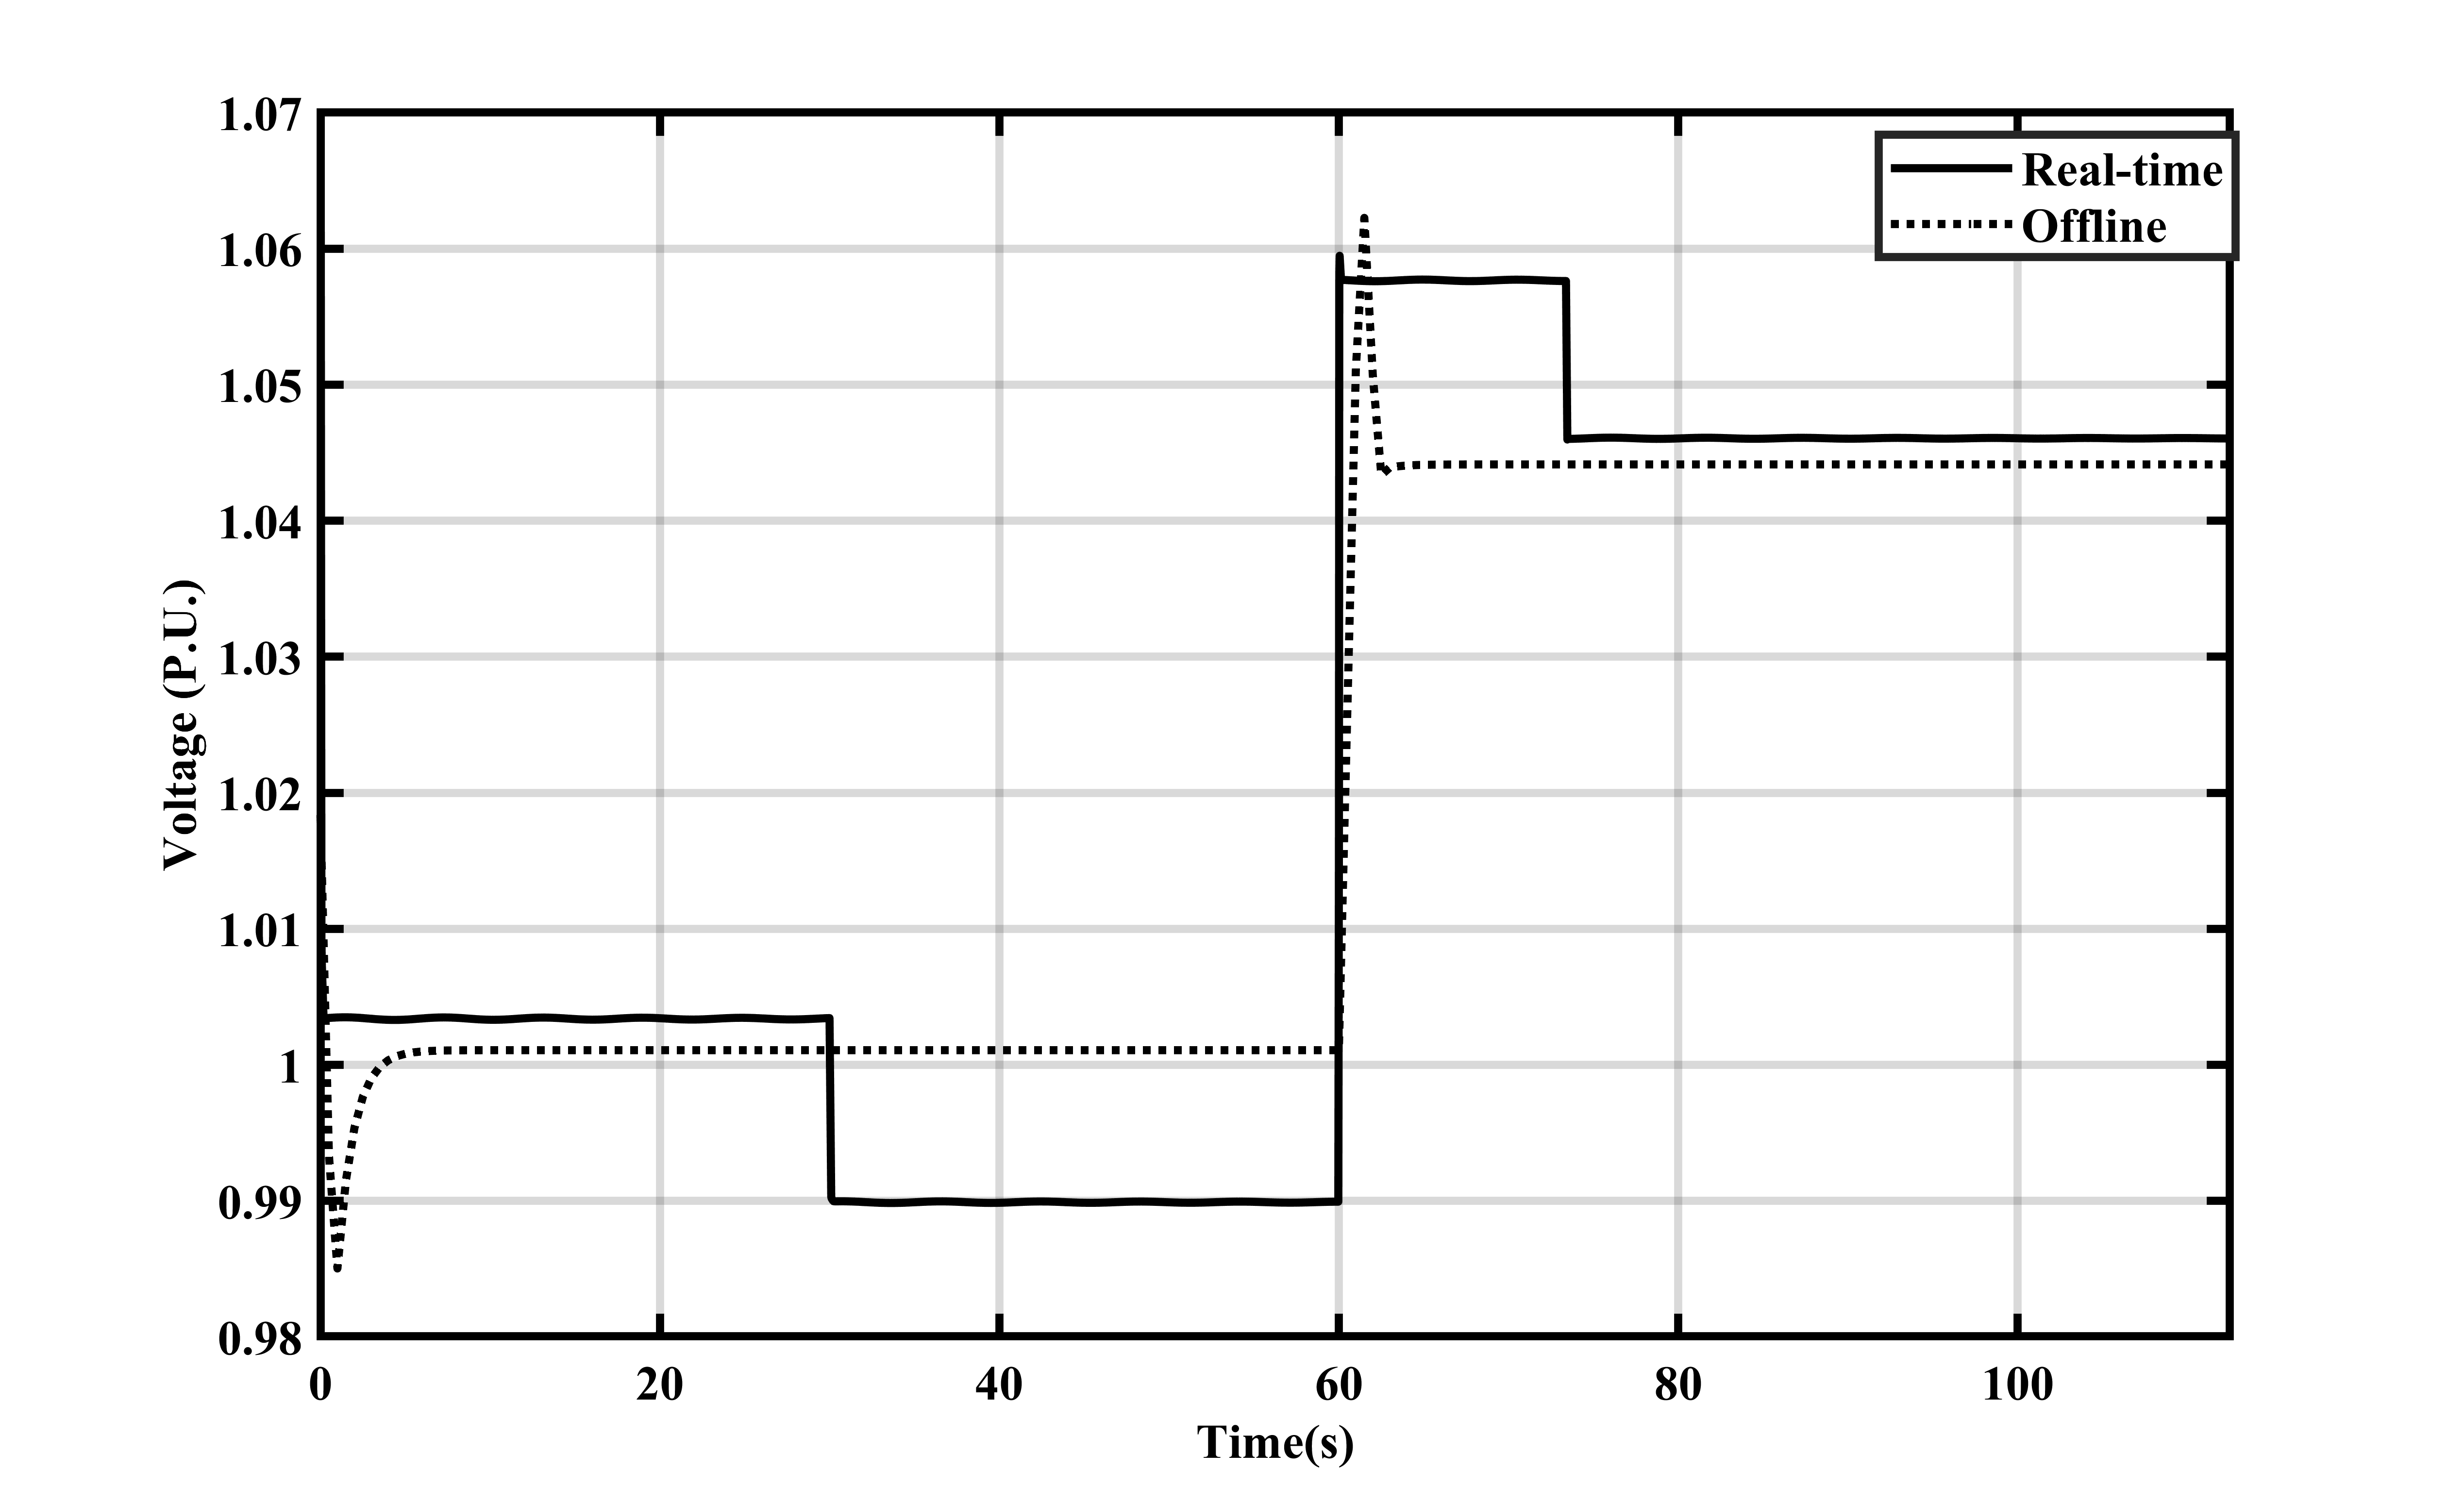
\includegraphics[width=\linewidth]{figs/OFF_VS_RT.png}
\caption{Real-time vs offline voltage profile with coordinated voltage control.}
\label{fig:RT_VS_OFF_V}
\end{figure}
\subsubsection{Real-time vs offline reactive power applied by PV}
Fig. \ref{fig:RT_PQ} shows the reactive power supplied the PV in B20090P. The offline results are shown using the solid line and real-time results are represented using the dotted lines. The responses differ less than 2\% and real-time response is seen to take longer in this case as well. The delay is consistent with the delay seen in Fig. \ref{fig:RT_VS_OFF_V}.

\begin{figure}[!h]
\centering
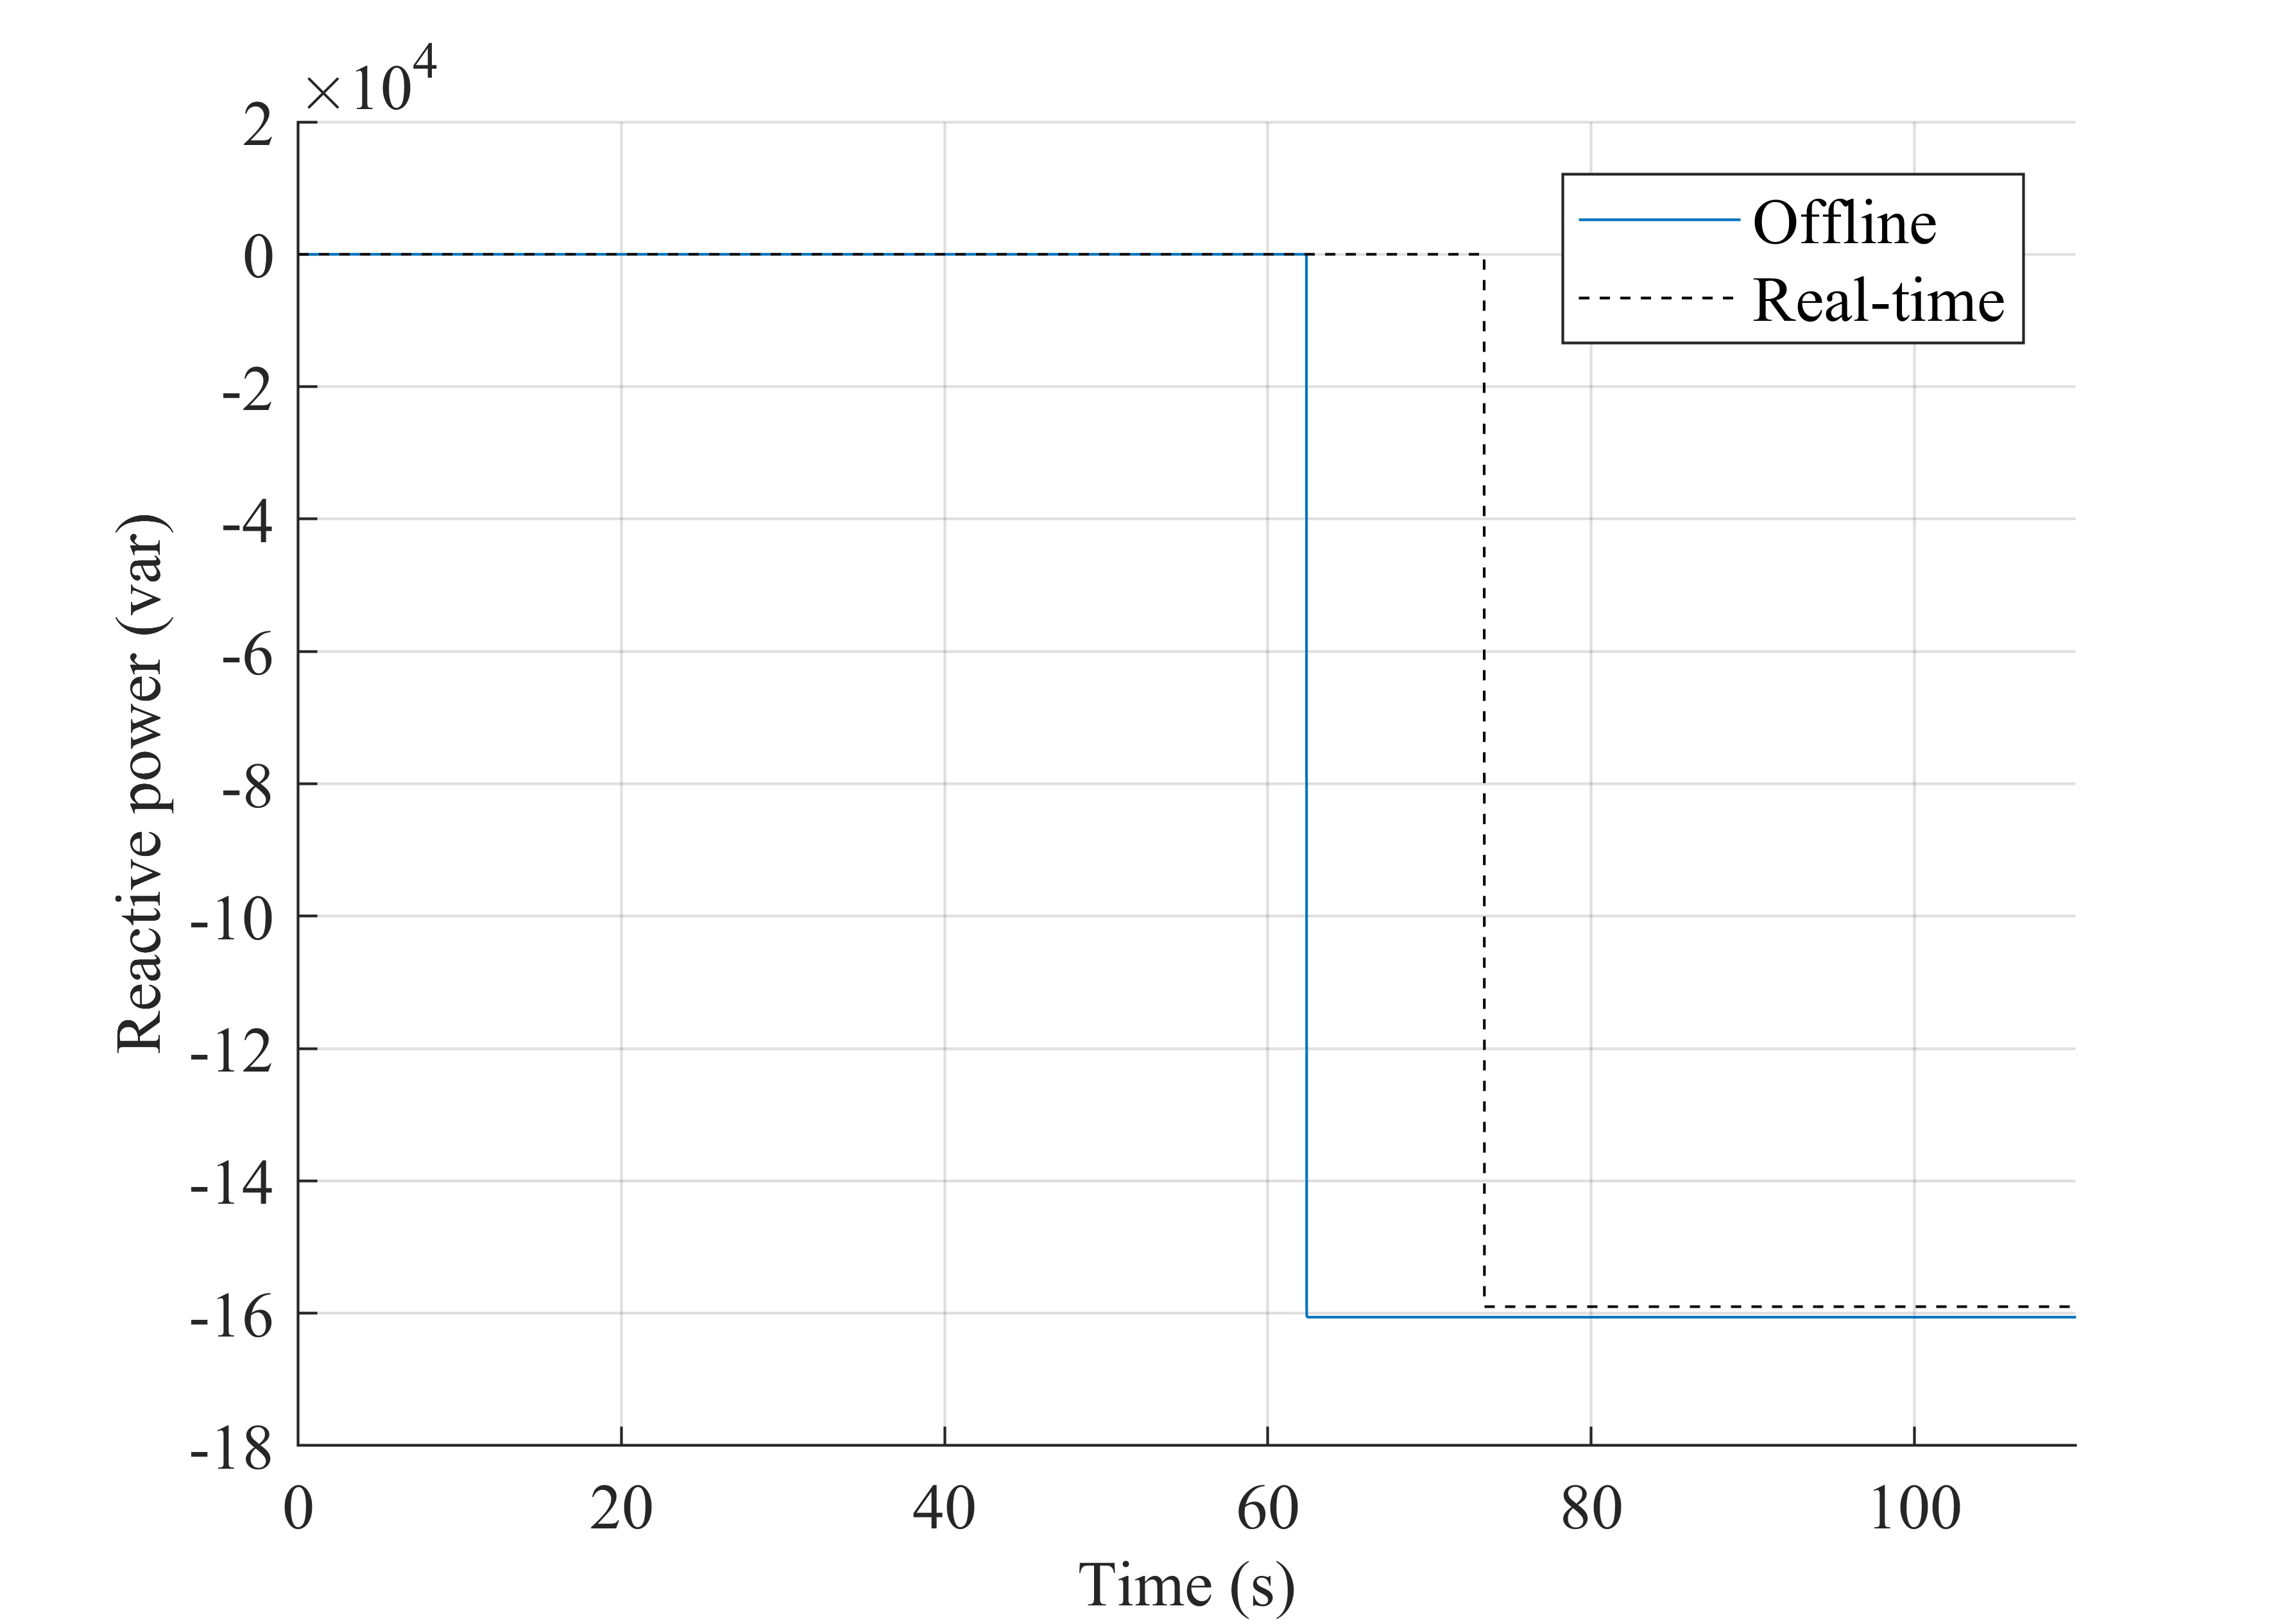
\includegraphics[width=\linewidth]{figs/PQ_RT.png}
\caption{Real-time vs off-line reactive power supplied by PV}
\label{fig:RT_PQ}
\end{figure}

\subsubsection{Real-time vs capacitor bank switching}
Finally, the switching operations of both CAP1 and CAP2 mentioned in Section \ref{off1} for both real-time and offline simulations are shown in Fig. \ref{fig:RT_CAP}. It can be seen that the responses are the same but the real-time response takes 13s. This is also contestant with the results shown in Fig. \ref{fig:RT_VS_OFF_V}.

\begin{figure}[!h]
\centering
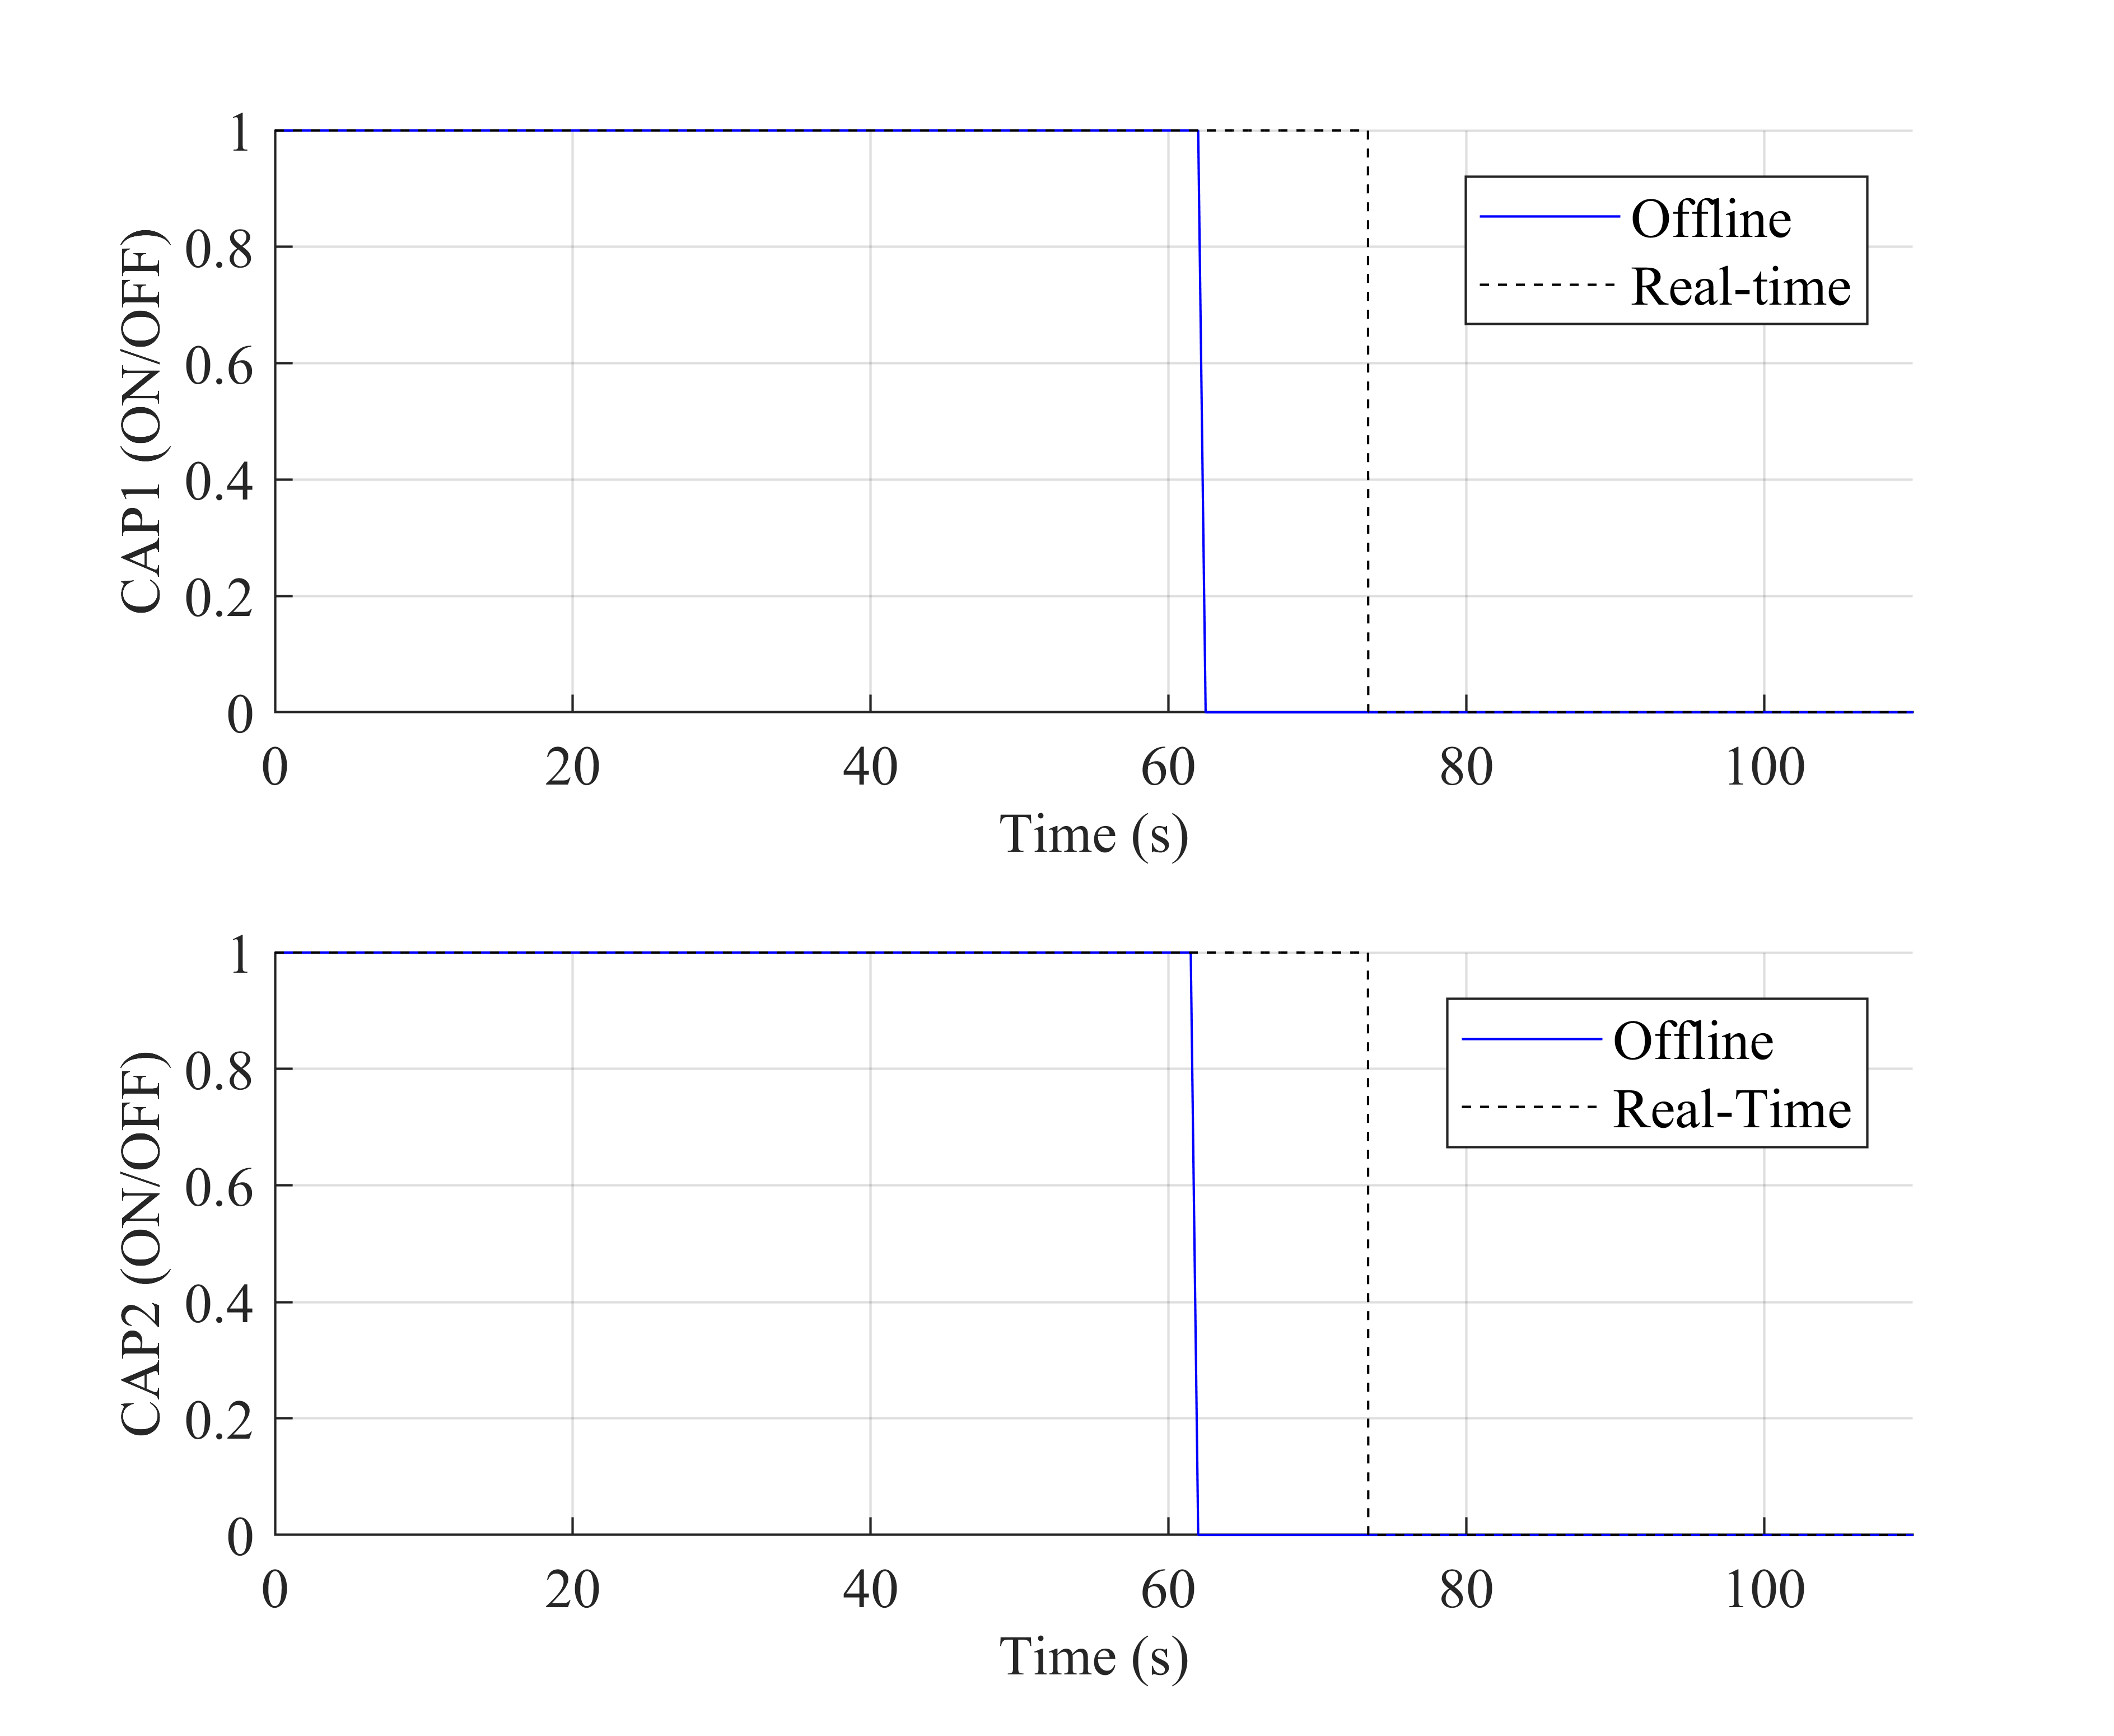
\includegraphics[width=\linewidth]{figs/CAPS_RT.PNG}
\caption{Capacitor bank switching states real-time vs offline.}
\label{fig:RT_CAP}
\end{figure}
